%----------------------------------------------------------------------------------------
% VLSP 2026 poster -- built on the a0poster portrait template (conference_poster_6.tex)
% Content follows the published paper: vlsp-pipeline/paper/acl/paper.pdf
% Build: pdflatex poster.tex   (run twice so citations resolve)
%----------------------------------------------------------------------------------------
\documentclass[a0,portrait]{a0poster}

\usepackage{multicol}
\columnsep=100pt
\columnseprule=3pt

\usepackage[svgnames]{xcolor}
\usepackage[utf8]{inputenc}
\usepackage[T5]{fontenc}   % Vietnamese letters in author names; text stays English
\usepackage{mathptmx}      % Times for text and maths
\usepackage{graphicx}
\graphicspath{{figures/}}
\usepackage{booktabs}
\usepackage{caption}
\DeclareCaptionFont{cap}{\fontsize{27}{32}\selectfont}
\captionsetup{font=cap,labelfont={bf,color=NavyBlue},textfont={color=Black!70}}
\usepackage{amsmath}
\usepackage{url}
\usepackage{tikz}
\usetikzlibrary{arrows.meta,positioning,calc}

\renewcommand{\columnseprulecolor}{\color{NavyBlue!35}}
\renewcommand{\refname}{\fontsize{30}{34}\selectfont\color{NavyBlue}References}
\newcommand{\envi}{EN$\rightarrow$VI}
\newcommand{\vien}{VI$\rightarrow$EN}
\newcommand{\bodyfont}{\fontsize{29.5}{35.5}\selectfont}
\newcommand{\psec}[1]{\section*{\fontsize{46}{52}\selectfont\color{NavyBlue}#1}}  % one accent colour for headings
\newcommand{\subt}{\fontsize{24}{27}\selectfont}               % second line inside figure boxes
\newcommand{\tabfont}{\bodyfont}                               % tables at body size
\newcommand{\bigstat}[2]{\begin{minipage}[t]{0.48\linewidth}\centering
  {\fontsize{112}{112}\selectfont\bfseries #1}\\[0.4cm]{\fontsize{30}{36}\selectfont #2}\end{minipage}}
\newcommand{\smallstat}[3]{\begin{minipage}[t]{#1\linewidth}\centering
  {\fontsize{56}{60}\selectfont\bfseries #2}\\[0.3cm]{\fontsize{26}{31}\selectfont #3}\end{minipage}}

%--- figure styles (drawn at ~1000pt width, rescaled to the column) -----------------------
\tikzset{
  box/.style={draw=NavyBlue, fill=NavyBlue!7, rounded corners=8pt, line width=2.5pt,
              minimum width=285pt, minimum height=134pt, align=center,
              font=\fontsize{27}{31}\selectfont, inner sep=6pt},
  io/.style={box, draw=DarkSlateGray, fill=DarkSlateGray!10},
  nbox/.style={box, minimum width=220pt, minimum height=150pt},
  nio/.style={io, minimum width=220pt, minimum height=150pt},
  chip/.style={fill=NavyBlue!14, rounded corners=6pt, minimum width=176pt, minimum height=36pt,
               font=\fontsize{24}{24}\selectfont, inner sep=0pt},
  arr/.style={-{Latex[length=16pt,width=14pt]}, line width=3pt, draw=NavyBlue},
  darr/.style={arr, dashed, draw=DarkSlateGray},
  num/.style={circle, fill=NavyBlue, text=white, font=\fontsize{24}{24}\selectfont\bfseries,
              minimum size=40pt, inner sep=0pt},
  sub/.style={font=\fontsize{24}{27}\selectfont, text=DarkSlateGray}
}

\begin{document}
\bodyfont

%----------------------------------------------------------------------------------------
%	POSTER HEADER
%----------------------------------------------------------------------------------------
\noindent\begin{minipage}[b]{0.78\linewidth}
\VeryHuge \color{NavyBlue} \textbf{Rainbow Cookie at VLSP 2026:\\[14pt]Small Models, Long Laws} \color{Black}\\[0.5cm]
\huge\textit{Document-Level English--Vietnamese Legal MT under 3B Parameters}\\[0.9cm]
\fontsize{47}{57}\selectfont \textbf{Trần Đức Lâm, Lê Vân Anh, Phạm Thị Khánh Linh, Nguyễn Thị Hiền Trang}\\[0.4cm]
\fontsize{39}{47}\selectfont University of Engineering and Technology, Vietnam National University, Hanoi, Vietnam\\[0.3cm]
\large \texttt{tranduclam06@gmail.com, vananh9684@gmail.com, 24022385@vnu.edu.vn, 24022470@vnu.edu.vn}\\
\end{minipage}
%
\begin{minipage}[b]{0.21\linewidth}\raggedleft

\includegraphics[width=12cm]{figures/vlsp-2026-logo.png}\\
\end{minipage}

\vspace{0.35cm}

%----------------------------------------------------------------------------------------
%	RESULTS AT A GLANCE: headline numbers and the main comparison (numbers from the paper)
%----------------------------------------------------------------------------------------
\noindent\begin{minipage}[c]{0.41\linewidth}
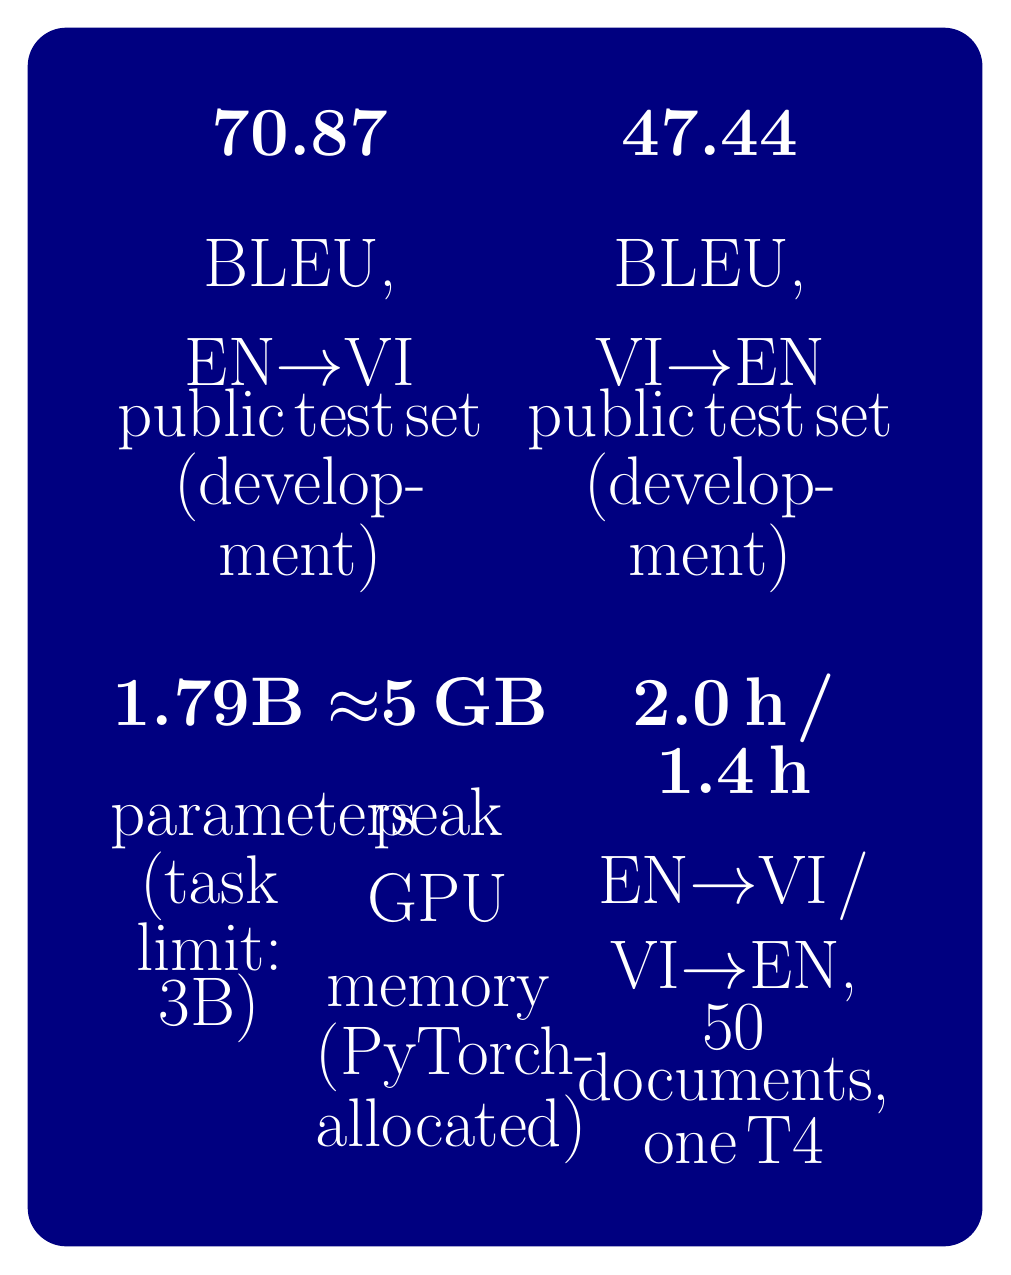
\begin{tikzpicture}
\node[fill=NavyBlue, text=white, rounded corners=14pt, inner xsep=30pt, inner ysep=30pt,
      text width=\dimexpr\linewidth-60pt\relax, align=center] {%
  \bigstat{70.87}{BLEU, \envi\\public test set (development)}\hfill
  \bigstat{47.44}{BLEU, \vien\\public test set (development)}\\[1.0cm]
  \smallstat{0.25}{1.79B}{parameters\\(task limit: 3B)}\hfill
  \smallstat{0.31}{$\approx$5\,GB}{peak GPU memory\\(PyTorch-allocated)}\hfill
  \smallstat{0.42}{2.0\,h / 1.4\,h}{\envi{} / \vien,\\50 documents, one T4}};
\end{tikzpicture}
\end{minipage}\hfill
\begin{minipage}[c]{0.56\linewidth}
\centering
\resizebox{\linewidth}{!}{%
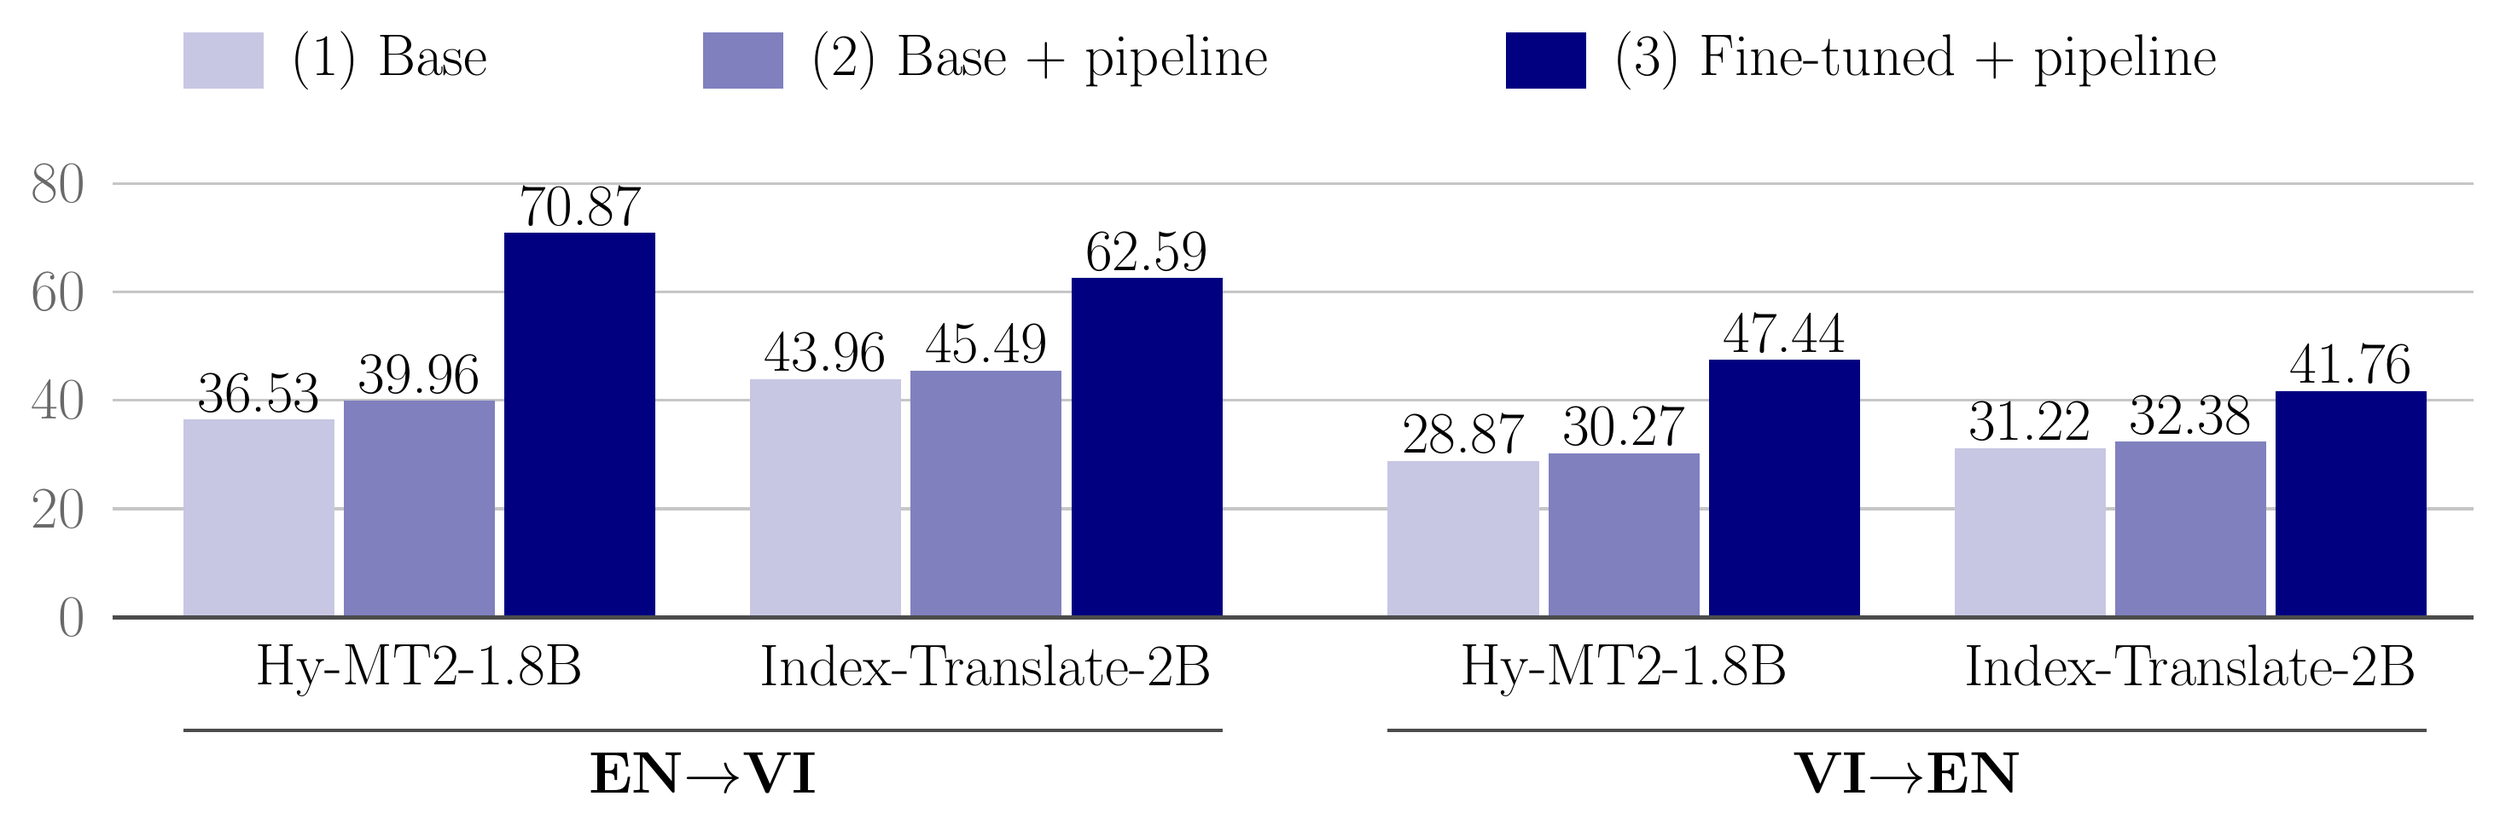
\begin{tikzpicture}[x=1pt,y=2.3pt]
\def\bw{64}
\foreach \v in {0,20,40,60,80}{
  \draw[Gray!45, line width=1.2pt] (0,\v) -- (1000,\v);
  \node[anchor=east, font=\fontsize{24}{24}\selectfont, text=DimGray] at (-8,\v) {\v};}
\foreach \x/\a/\b/\c in {30/36.53/39.96/70.87, 270/43.96/45.49/62.59, 540/28.87/30.27/47.44, 780/31.22/32.38/41.76}{
  \foreach \i/\v/\col in {0/\a/NavyBlue!22, 1/\b/NavyBlue!50, 2/\c/NavyBlue}{
    \fill[\col] (\x+\i*68,0) rectangle (\x+\i*68+\bw,\v);
    \node[anchor=south, inner sep=3pt, font=\fontsize{23}{23}\selectfont] at (\x+\i*68+32,\v) {\v};}}
\draw[Black!70, line width=2pt] (0,0) -- (1000,0);
\foreach \x/\m in {130/Hy-MT2-1.8B, 370/Index-Translate-2B, 640/Hy-MT2-1.8B, 880/Index-Translate-2B}
  \node[anchor=north, font=\fontsize{25}{25}\selectfont] at ([yshift=-8pt]\x,0) {\m};
\foreach \l/\r/\d in {30/470/\envi, 540/980/\vien}{
  \draw[Black!70, line width=1.5pt] ([yshift=-48pt]\l,0) -- ([yshift=-48pt]\r,0);
  \node[anchor=north, yshift=-54pt, font=\fontsize{27}{27}\selectfont\bfseries] at ({(\l+\r)/2},0) {\d};}
\foreach \x/\col/\t in {30/NavyBlue!22/(1) Base, 250/NavyBlue!50/(2) Base + pipeline, 590/NavyBlue/(3) Fine-tuned + pipeline}{
  \fill[\col] ([yshift=40pt]\x,80) rectangle ([yshift=64pt]\x+34,80);
  \node[anchor=west, font=\fontsize{25}{25}\selectfont] at ([yshift=52pt]\x+42,80) {\t};}
\end{tikzpicture}}
\captionof{figure}{SacreBLEU~\cite{post2018sacrebleu} on the public test set (50 documents). The two (1) bars are not directly comparable: Hy-MT2 is sampled (3-seed mean), Index is greedy.}
\end{minipage}

\vspace{0.35cm}

\color{Black!88}
\begin{multicols}{2}

%----------------------------------------------------------------------------------------
%	INTRODUCTION
%----------------------------------------------------------------------------------------
\psec{Task and Challenges}

\begin{itemize}
\item \textbf{Fidelity:} terminology, obligations and exceptions must survive translation.
\item \textbf{Structure:} numbered articles, nested clauses and tables, in documents longer than the model context.
\item \textbf{Constraints:} $<$3B parameters, fully local, no external API~\cite{vlsp2026}; \textbf{time} and \textbf{memory} are scored.
\end{itemize}

%----------------------------------------------------------------------------------------
%	DATA
%----------------------------------------------------------------------------------------
\psec{1. Training Data Processing}

Documents are sliced at preamble, article, clause and document boundaries; a row pairs a slice with its translation: \textbf{54,134 rows (575 documents)} become \textbf{82,203 rows (612 documents)}.

\begin{center}
\resizebox{\linewidth}{!}{%
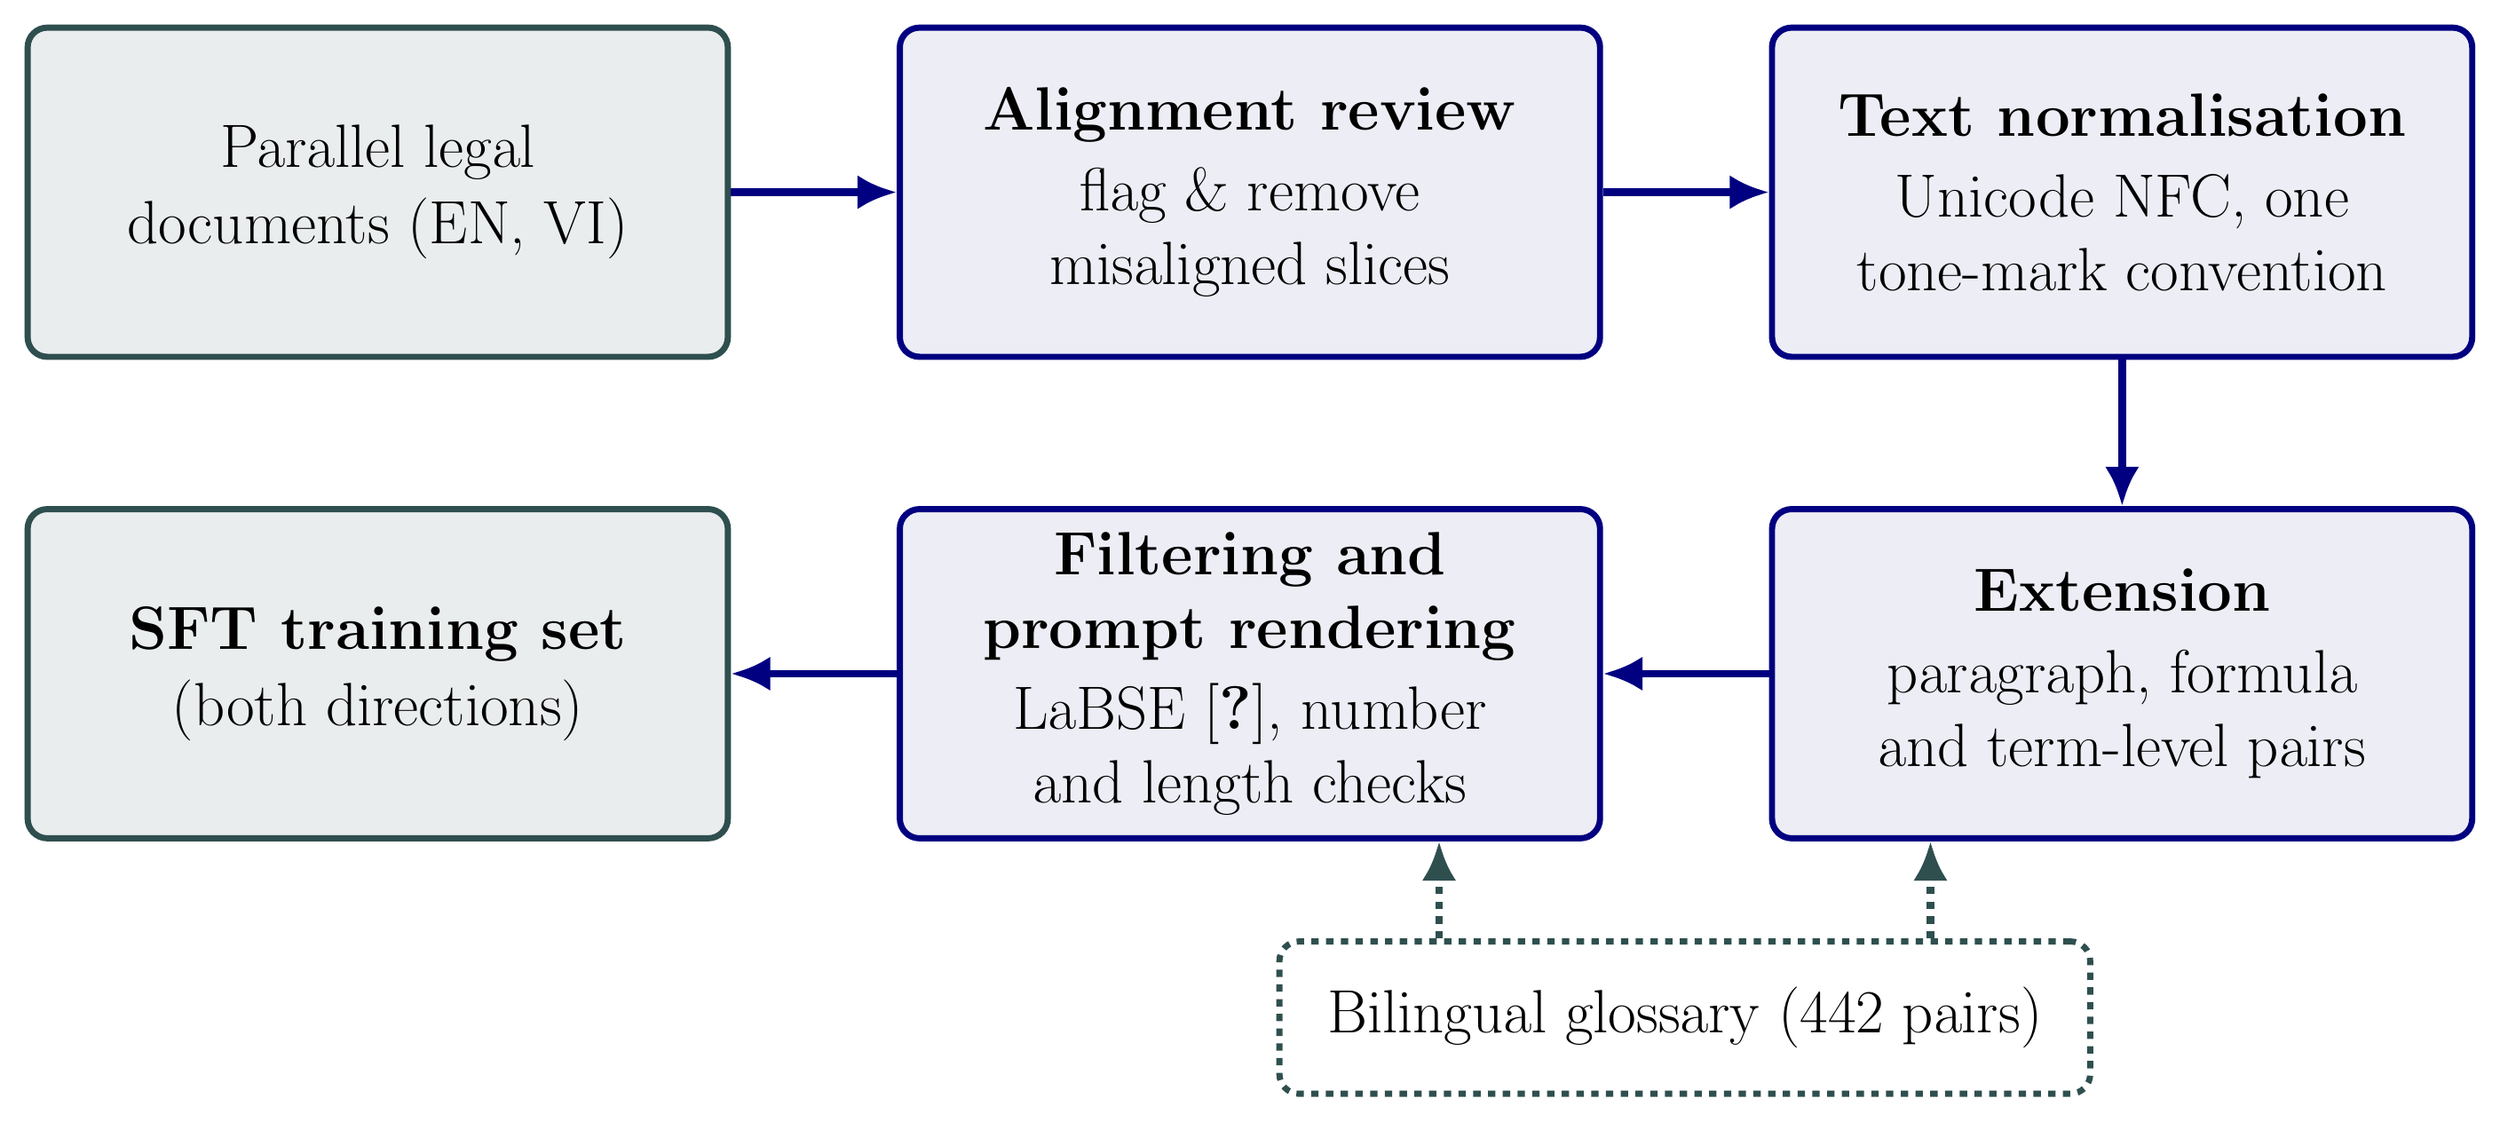
\begin{tikzpicture}[x=1pt,y=1pt]
\node[io]  (a) at (0,0)      {Parallel legal\\documents (EN, VI)};
\node[box] (b) at (355,0)    {\textbf{Alignment review}\\[2pt]\subt flag \& remove\\[-1pt]\subt misaligned slices};
\node[box] (c) at (710,0)    {\textbf{Text normalisation}\\[2pt]\subt Unicode NFC, one\\[-1pt]\subt tone-mark convention};
\node[box] (d) at (710,-196) {\textbf{Extension}\\[2pt]\subt paragraph, formula\\[-1pt]\subt and term-level pairs};
\node[box] (e) at (355,-196) {\textbf{Filtering and}\\[-1pt]\textbf{prompt rendering}\\[2pt]\subt LaBSE~\cite{feng2022labse}, number\\[-1pt]\subt and length checks};
\node[io]  (f) at (0,-196)   {\textbf{SFT training set}\\(both directions)};
\node[draw=DarkSlateGray, dashed, line width=2.5pt, rounded corners=8pt, minimum width=330pt, minimum height=62pt,
      font=\fontsize{25}{25}\selectfont] (g) at (532,-336) {Bilingual glossary (442 pairs)};
\draw[arr] (a) -- (b);
\draw[arr] (b) -- (c);
\draw[arr] (c) -- (d);
\draw[arr] (d) -- (e);
\draw[arr] (e) -- (f);
\draw[darr] ([xshift=100pt]g.north) -- ([xshift=100pt]g.north |- d.south);
\draw[darr] ([xshift=-100pt]g.north) -- ([xshift=-100pt]g.north |- e.south);
\end{tikzpicture}}
\captionof{figure}{Preparation of the supervised fine-tuning corpus.}
\end{center}

\begin{itemize}
\item \textbf{Alignment:} 237 slices flagged, \textbf{158 excluded} after manual review.
\item \textbf{Normalisation:} NFC, look-alike characters, one tone-mark convention; same at inference.
\item \textbf{Glossary:} \emph{training-only} hints in 19,495 rows (23.7\%); none at inference.
\item \textbf{Composition:} 50,129 original rows after cleaning, 30,658 paragraph-level, 654 hand-written formula and 762 terminology rows.
\item \textbf{Sources:} organiser data and author-written rows only, no external corpora. All 41 development documents are merged into training; 23 other held-out documents serve only for validation loss.
\end{itemize}


%----------------------------------------------------------------------------------------
%	FINE-TUNING
%----------------------------------------------------------------------------------------
\psec{2. Base Models and Fine-Tuning}

\begin{itemize}
\item \textbf{Models:} Hy-MT2-1.8B~\cite{zheng2026hymt2} and Index-Translate-2B~\cite{indexteam} with LoRA~\cite{hu2022lora}; base weights frozen.
\item \textbf{LoRA:} rank 64, $\alpha$ = 128 on attention and MLP projections: \textbf{77.6M} trainable parameters (4.15\%).
\item \textbf{Training:} loss on response tokens only; two passes ($\sim$53.5k, then 82,203 rows). Adapters are merged for inference (\textbf{1.79B} parameters).
\end{itemize}

\columnbreak

%----------------------------------------------------------------------------------------
%	PIPELINE
%----------------------------------------------------------------------------------------
\psec{3. Document-Level Pipeline}

\begin{center}
\resizebox{\linewidth}{!}{%
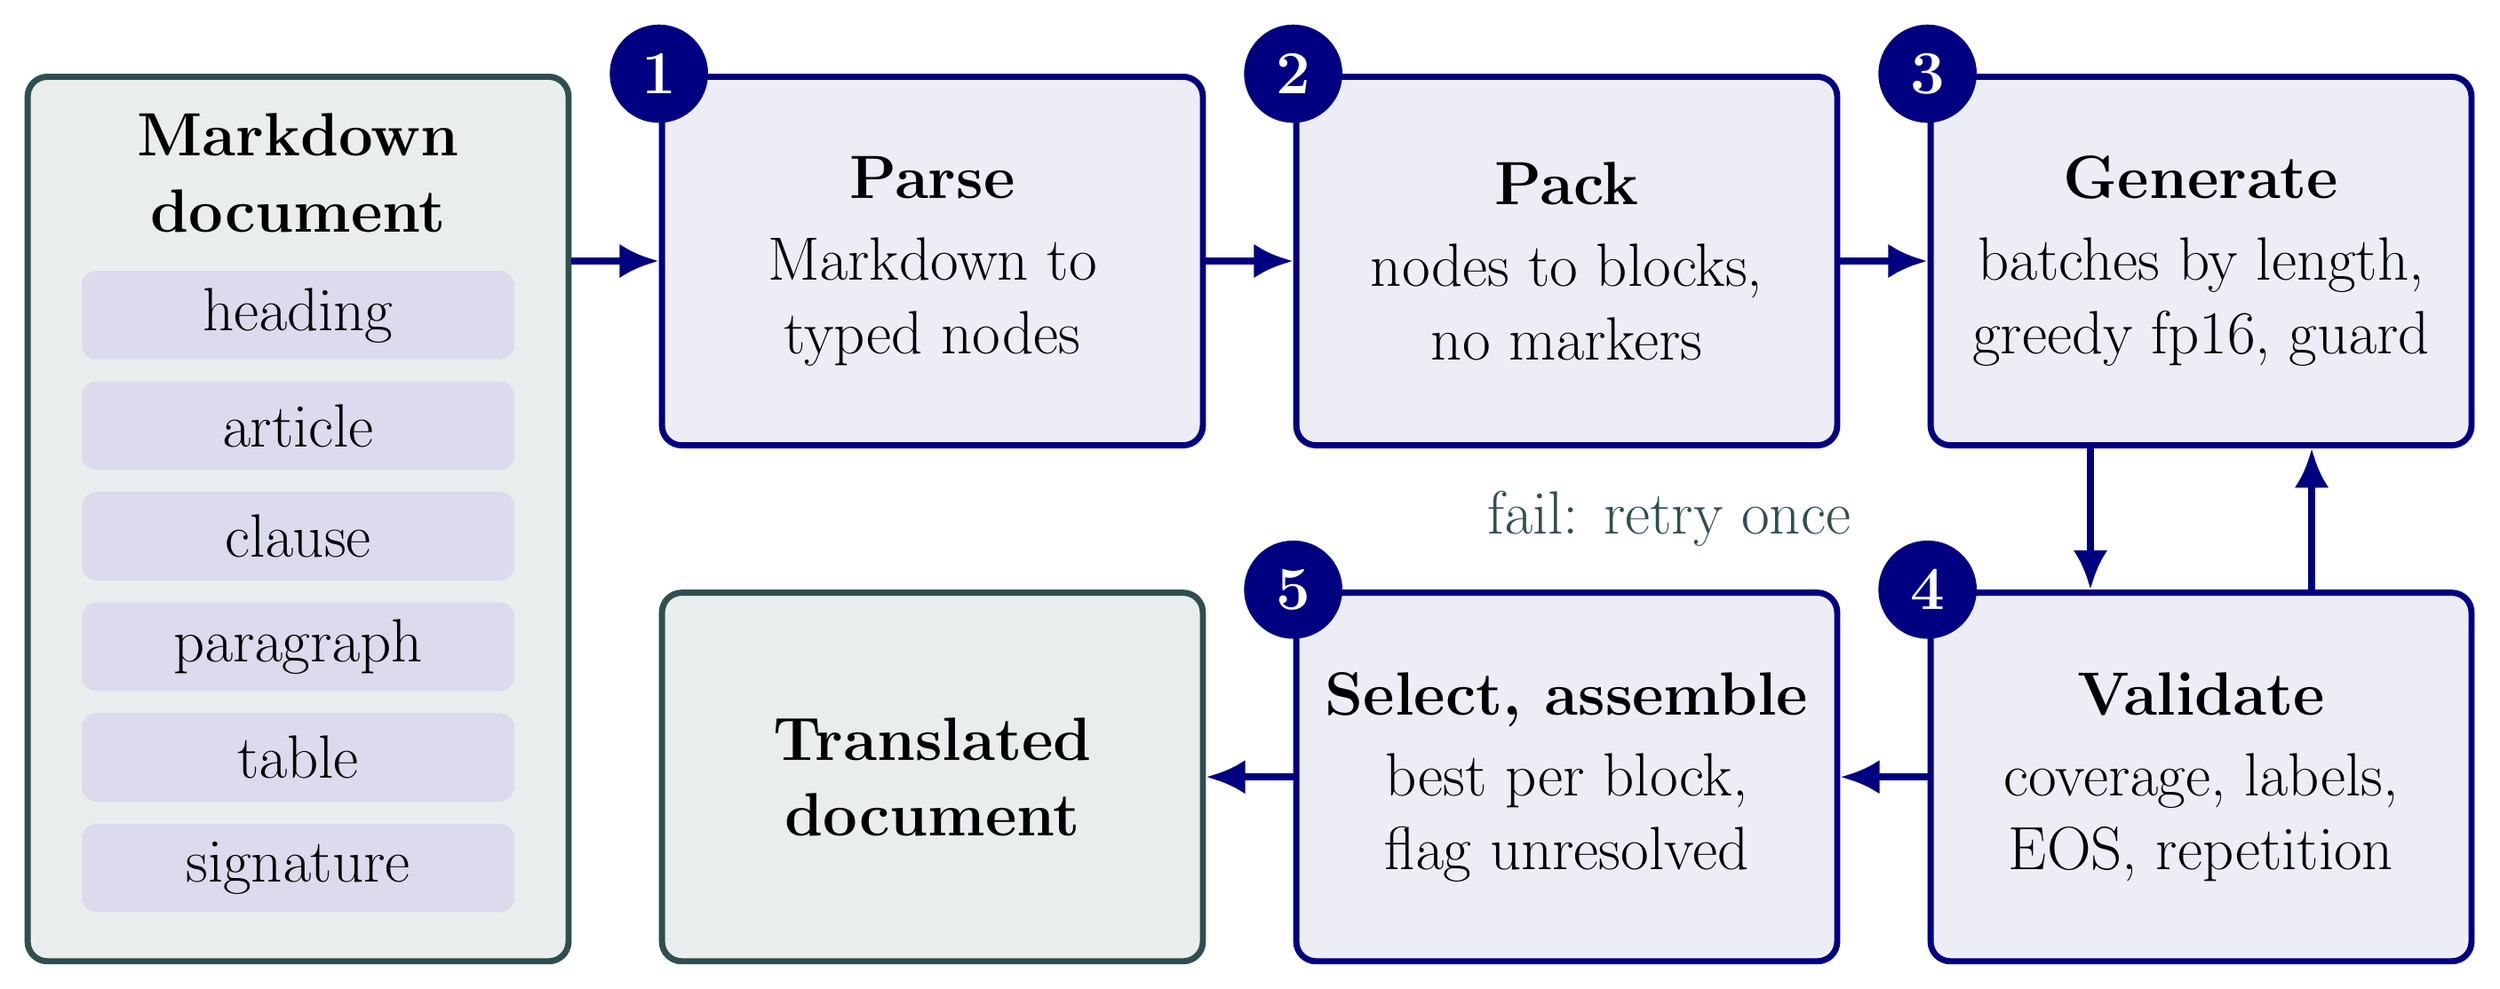
\begin{tikzpicture}[x=1pt,y=1pt]
\node[io, minimum width=220pt, minimum height=360pt] (in) at (110,-105) {};
\node[font=\fontsize{27}{31}\selectfont\bfseries, align=center] at (110,36) {Markdown\\document};
\foreach \t [count=\i] in {heading,article,clause,paragraph,table,signature}
  \node[chip] at (110,{-22-(\i-1)*45}) {\t};
\node[nbox] (p) at (368,0)    {\textbf{Parse}\\[2pt]\subt Markdown to\\[-1pt]\subt typed nodes};
\node[nbox] (k) at (626,0)    {\textbf{Pack}\\[2pt]\subt nodes to blocks,\\[-1pt]\subt no markers};
\node[nbox] (g) at (884,0)    {\textbf{Generate}\\[2pt]\subt batches by length,\\[-1pt]\subt greedy fp16, guard};
\node[nbox] (v) at (884,-210) {\textbf{Validate}\\[2pt]\subt coverage, labels,\\[-1pt]\subt EOS, repetition};
\node[nbox] (s) at (626,-210) {\textbf{Select, assemble}\\[2pt]\subt best per block,\\[-1pt]\subt flag unresolved};
\node[nio]  (o) at (368,-210) {\textbf{Translated}\\\textbf{document}};
\node[num] at (p.north west) {1};
\node[num] at (k.north west) {2};
\node[num] at (g.north west) {3};
\node[num] at (v.north west) {4};
\node[num] at (s.north west) {5};
\draw[arr] (in.east |- p.west) -- (p.west);
\draw[arr] (p) -- (k);
\draw[arr] (k) -- (g);
\draw[arr] ([xshift=-45pt]g.south) -- ([xshift=-45pt]v.north);
\draw[arr] ([xshift=45pt]v.north) -- ([xshift=45pt]g.south);
\node[sub, anchor=east] at ([xshift=-139pt]$(g.south)!0.5!(v.north)$) {fail: retry once};
\draw[arr] (v) -- (s);
\draw[arr] (s) -- (o);
\end{tikzpicture}}
\captionof{figure}{Structured translation with one selective recovery round.}
\end{center}

\begin{itemize}
\item \textbf{Parse and pack:} a rule-based parser keeps a lossless partition; adjacent prose is joined by newlines, \emph{no markers}, in blocks of $\sim$768 tokens or 8 nodes.
\item \textbf{Validate:} hard failures include empty output, missing EOS, lost labels and severe repetition. Checks are structural, not semantic.
\item \textbf{Recover once:} failed units are retried in sentence-preserving pieces.
\end{itemize}

\begin{center}
\begin{tikzpicture}
\node[fill=DarkSlateGray!7, draw=DarkSlateGray!60, line width=2pt, rounded corners=10pt, inner xsep=22pt, inner ysep=18pt,
      text width=\dimexpr\linewidth-48pt\relax, align=left, font=\fontsize{27}{33}\selectfont] {%
  {\bfseries\color{NavyBlue} Example: a lost clause label triggers recovery}\\[10pt]
  \begin{minipage}[t]{0.21\linewidth}\textbf{Source block}\\Article 5. \dots\\1. \dots\\2. \dots\end{minipage}\hfill
  \begin{minipage}[t]{0.27\linewidth}\textbf{First output}\\Điều 5. \dots\\1. \dots\\\dots\ \ \textcolor{Crimson}{\textbf{label ``2.'' lost}}\end{minipage}\hfill
  \begin{minipage}[t]{0.45\linewidth}\textbf{Validate and recover}\\Hard failure: a protected label is missing. Retry in smaller pieces, with an instruction to keep the listed labels.\end{minipage}};
\end{tikzpicture}
\end{center}

%----------------------------------------------------------------------------------------
%	RESULTS
%----------------------------------------------------------------------------------------
\psec{4. Results (Public Test Set, 50 Documents)}

\begin{itemize}
\item \textbf{Fine-tuning gives the largest observed gain:} 39.96 $\to$ 70.87 (\envi) and 30.27 $\to$ 47.44 (\vien); chrF 84.48 / 79.50. Data cleaning is not ablated separately.
\item \textbf{Model choice:} Index is stronger before fine-tuning (45.49 vs.\ 39.96, \envi), Hy-MT2 after it (70.87 vs.\ 62.59).
\item \textbf{Pipeline:} +1.53 / +1.16 BLEU for Index at fixed greedy decoding. For Hy-MT2, (1)$\to$(2) also changes sampling to greedy.
\item \textbf{Grouping} (earlier checkpoint, $\sim$53.5k rows, one run each): blocks without markers reach 68.90 / 46.62 BLEU against 67.69 / 45.23 for separate requests (paired 95\% CIs exclude 0); the gain over markers is uncertain for \vien.
\item \textbf{Recovery} re-translates 4.8\% / 10.6\% of units; 0.9\% / 6.7\% stay unresolved (11 and 29 documents): structural failures, mostly lost labels, not omission rates.
\item \textbf{Uncertainty:} final BLEU 95\% CIs are [65.68, 74.24] and [42.30, 50.99]; they reflect document sampling, not training-seed variance.
\end{itemize}

\begin{center}
\tabfont
\begin{tabular*}{\linewidth}{@{\extracolsep{\fill}}l c c c c@{}}
\toprule
 & \multicolumn{2}{c}{Time (s)} & \multicolumn{2}{c}{GPU alloc. (GB)} \\
\cmidrule(lr){2-3}\cmidrule(lr){4-5}
\textbf{Hy-MT2-1.8B} & \envi & \vien & \envi & \vien \\
\midrule
(1) Base, per seed & $\sim$4.0k & $\sim$4.1k & 5.41 & 4.90 \\
(2) Base + pipeline & 8,111 & 5,326 & 5.34 & 5.15 \\
(3) Fine-tuned + pipeline & 7,229 & 4,871 & 4.96 & 5.25 \\
\bottomrule
\end{tabular*}
\captionof{table}{One T4 per direction. PyTorch-allocated peak; process-level usage is higher.}
\end{center}

\begin{itemize}
\item \textbf{Not reported:} private-test scores, legal-accuracy, terminology or neural metrics. \vien{} stays below \envi{} in BLEU for every system.
\end{itemize}

\end{multicols}

\vspace{0.3cm}
\noindent\begin{tikzpicture}
\node[fill=NavyBlue!8, draw=NavyBlue, line width=2.5pt, rounded corners=14pt, inner xsep=30pt, inner ysep=14pt,
      text width=\dimexpr\linewidth-65pt\relax, align=left] {%
  \begin{minipage}[t]{0.52\linewidth}
  {\color{NavyBlue}\bfseries Conclusion.} Legal-domain LoRA adaptation of Hy-MT2-1.8B plus structured Markdown translation with selective recovery reaches \textbf{70.87 / 47.44 BLEU} (\envi{} / \vien{}) at about 5~GB and 2.0 / 1.4 h per direction on a T4. These are development results; independent legal-accuracy and generalisation evaluation remains necessary.
  \end{minipage}\hfill
  \begin{minipage}[t]{0.45\linewidth}\fontsize{19}{21.5}\selectfont
  \renewcommand{\section}[2]{}%
  \begin{thebibliography}{9}\setlength{\itemsep}{0pt}\setlength{\parskip}{0pt}
  \bibitem{vlsp2026} VLSP 2026 Organizers, ``Document-level legal machine translation with limited-parameter models,'' 2026. \url{https://vlsp.org.vn/vlsp2026/eval/mt_challenge}
  \bibitem{zheng2026hymt2} M. Zheng et al., ``Hy-MT2: A family of fast, efficient and powerful multilingual translation models in the wild,'' arXiv:2605.22064, 2026.
  \bibitem{indexteam} T. Li et al., ``Index-Translate: A multilingual translation model family,'' arXiv:2609.40181, 2026.
  \bibitem{hu2022lora} E. J. Hu et al., ``LoRA: Low-rank adaptation of large language models,'' ICLR 2022.
  \bibitem{feng2022labse} F. Feng et al., ``Language-agnostic BERT sentence embedding,'' ACL 2022.
  \bibitem{post2018sacrebleu} M. Post, ``A call for clarity in reporting BLEU scores,'' WMT 2018.
  \end{thebibliography}
  \end{minipage}};
\end{tikzpicture}

\end{document}
